% -----------------------------*- LaTeX -*------------------------------
\documentclass[11pt]{report}
\usepackage{scribe_ds603}
\usepackage{amsthm}

\theoremstyle{remark}
\newtheorem*{remark}{Remark}

\DeclareMathAlphabet{\stdmathcal}{OMS}{cmsy}{m}{n}

\begin{document}


\scribe{Suhas Rao}		% required
\lecturenumber{10}			% required, must be a number
\lecturedate{24th September}		% required, omit year

\maketitle

% ----------------------------------------------------------------------


\section{Attack Strategy}
This lecture explores additional attack strategies, building upon the concepts of Label Flipping and Bilevel Optimization discussed previously. We will now delve into Feature Collision and Gradient Alignment attacks.

\subsection{Feature Collision}
\textbf{Threat Model:} The Feature Collision attack is a targeted poisoning attack executed in either a clean-label or backdoor  attack setting. This strategy assumes the attacker has access to both the training data and the model, with the model being pre-trained and only subject to fine-tuning.\\
\\
\textbf{Attack:} An attacker first chooses a $target\, instance$ from the test set; a successful poisoning attack causes this target example to be misclassified during test time. Next, the attacker samples a $base\, instance$ from
the base class and makes imperceptible changes to it to craft a $poison\, instance$; this poison is injected into the training data with the intent of fooling the model into labeling the target instance with the base label at test time. Finally, the model is trained on the poisoned dataset (clean dataset + poison instances). If, at test time, the model mistakes the target instance as being in the base class, then the poisoning attack is considered successful.

Let $\phi: \mathbb{R}^k \rightarrow \mathbb{R}^s$ be the feature extractor of the model, which is known to the attacker. The attacker's objective is to craft a poison instance $\Vec{x}\,^p$ that is close to a base instance $\Vec{x}\,^b$ in the input space, while its feature representation $\phi(\Vec{x}\,^p)$ is close to the feature representation of the target instance $\Vec{x}\,^t$. This can be formulated as an optimization problem:
\[\Vec{x}\,^p = \argmin_{\Vec{x}\,\in \,\stdmathcal{X}} \, \norm{\phi(\Vec{x})-\phi(\Vec{x}\,^{t})}^2_2 + \lambda\norm{\Vec{x}-\Vec{x}\,^b}^2_2\]
Here, $\lambda$ is a regularization parameter that balances the two competing objectives.

Let $h : \Rbb^k \ra \stdmathcal{Y}$ be the model where $h(\Vec{x})=c(\phi(\Vec{x}))=y \,\in \stdmathcal{Y}$ such that $c(\cdot)$ alone is allowed to be retrained.
\begin{itemize}
    \item[1.]\textbf{Clean Model:}\\
    On a clean model,\, $h(\Vec{x}\,^p) = y\,^t$, since $\phi(\Vec{x}\,^p)$ is close to $\phi(\Vec{x}\,^t)$ in the representation space and $h(\Vec{x}\,^t) = y\,^t$.
    \item[2.]\textbf{Poisoned Model:}\\
    On a poisoned model, which is retrained with the poison instances,\, $h(\Vec{x}\,^p) = y\,^b$ since $\Vec{x}\,^p$ is close to $\Vec{x}\,^b$ in the input space. As the decision boundary of the model has been modified, it is possible that\, $h(\Vec{x}\,^t) = y\,^b$. Then the poisoning attack is considered successful.
\end{itemize}

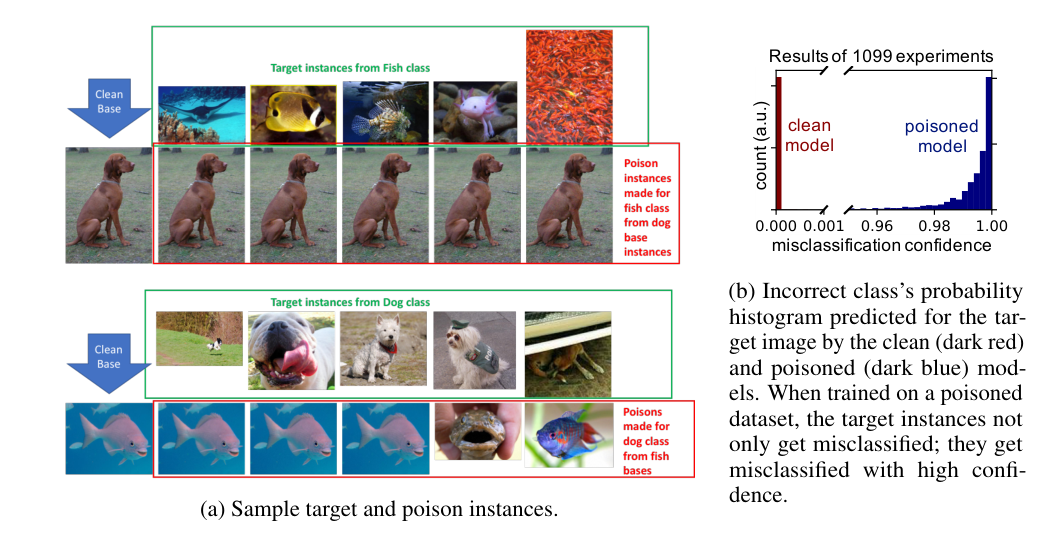
\includegraphics[width=\linewidth]{images/feature_collision.png}

\subsection{Gradient Alignment}
\textbf{Threat Model:} This is a targeted poisoning attack in clean and backdoor attack setup where both data and model access is assumed.\\
\\
\textbf{Attack:} If attacker could insert target image $\Vec{x}\,^t$ into the training set, and label it as $y\,^{adv}$, then there's nothing to do, as the model will learn to label adversarially to minimize training loss. Hence, here we are assuming the attacker is not able to insert the mis-labeled target. So, the goal is to mimic the gradient of the target by creating posioned data whose gradient correlates with the adversarial target gradient.

Let $\stdmathcal{L}(D_p, \Vec{\theta})$ be the loss on a batch of poison data $D_p$ with model parameters $\Vec{\theta}$, and let $\ell(h_{\Vec{\theta}}(\Vec{x}\,^t, y\,^{adv}), \Vec{\theta})$ be the loss for the target instance with the adversarial label. The objective is to maximize the cosine similarity between the gradients of these two losses. This can be expressed as minimizing the following objective function $\stdmathcal{B}(D_p, \Vec{\theta})$:
\[
\stdmathcal{B}(D_p, \Vec{\theta}) = 1 -
\frac{
    \left\langle 
        \nabla_{\Vec{\theta}} \ell(h_{\Vec{\theta}}(\Vec{x}\,^t, y\,^{adv}), {\Vec{\theta}}),
        \nabla_{\Vec{\theta}} \hat{\stdmathcal{L}}(D_p, {\Vec{\theta}})
    \right\rangle
}{
    \|\nabla_{\Vec{\theta}} \ell(h_{\Vec{\theta}}(\Vec{x}\,^t, y\,^{adv}), {\Vec{\theta}})\|
    \cdot
    \left\|
        \nabla_{\Vec{\theta}} \hat{\stdmathcal{L}}(D_p, {\Vec{\theta}})
    \right\|
}.
\]

By minimizing this value, the attacker ensures that when the model is trained on the poison data to minimize $\stdmathcal{L}(D_p, \Vec{\theta})$, it will also inadvertently minimize the loss on the target instance with the adversarial label, leading to the desired misclassification.


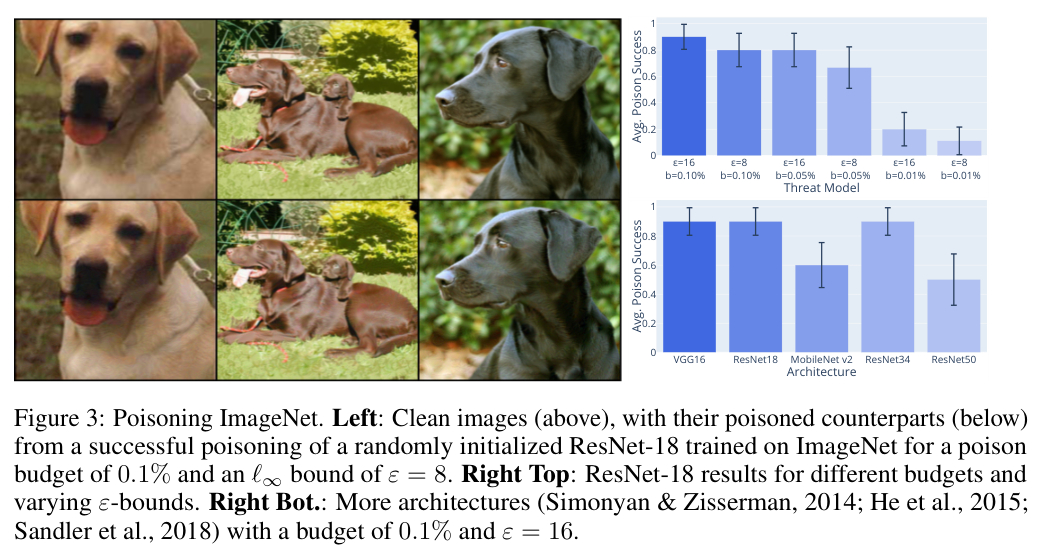
\includegraphics[width=\linewidth]{images/gradient_alignment.png}

\begin{remark}
    Poisons are tested on a newly initialized model of the same architecture.
\end{remark}

\section{Attack Realism}

\subsection{Black Box Attacks}
In a black-box attack setting, the adversary has limited knowledge about the target model. They do not have access to the model's architecture, parameters, or training data. The only capability is to query the model with inputs and observe the corresponding outputs (labels).

A common strategy for black-box attacks is to train a \textit{substitute model}. The attacker creates a synthetic dataset and labels it by querying the target model. This dataset is then used to train a local model that mimics the behavior of the target model. Adversarial examples are then crafted for this substitute model, with the hope that they will also be effective against the original target model due to a phenomenon known as \textit{attack transferability}.


\subsection{Physical Triggers}
An attacker launches backdoor attacks against a Deep Neural Network in two steps. During model training, the attacker poisons the training dataset by adding samples associating inputs containing a chosen pattern (the trigger $\delta$) with a target label $y_t$. This produces a backdoored model that correctly classifies benign inputs but “misclassifies” any input containing the trigger $\delta$ to the target label $y_t$. At inference time, the attacker activates the backdoor by adding the trigger $\delta$ to any input, forcing the model to classify the input as $y_t$.

Empirically, such attacks are highly effective even with low poisoning rates (around 15--25\%), achieving high attack success while preserving clean accuracy. The effectiveness depends on the trigger's location and visibility: triggers placed over salient regions (e.g., facial features) succeed far more often than those placed peripherally. Furthermore, these attacks are robust to variations such as lighting, blur, compression, and noise, and often transfer across different model architectures.

Defenses developed for digital backdoor attacks such as Neural Cleanse, Spectral Signatures, Activation Clustering, and STRIP struggle against physical triggers. Since physical objects produce feature activations that resemble clean data, these methods often fail to isolate or detect the backdoor. Consequently, physical backdoor attacks represent a realistic and persistent threat, emphasizing the need for defenses explicitly designed for physically realizable triggers.

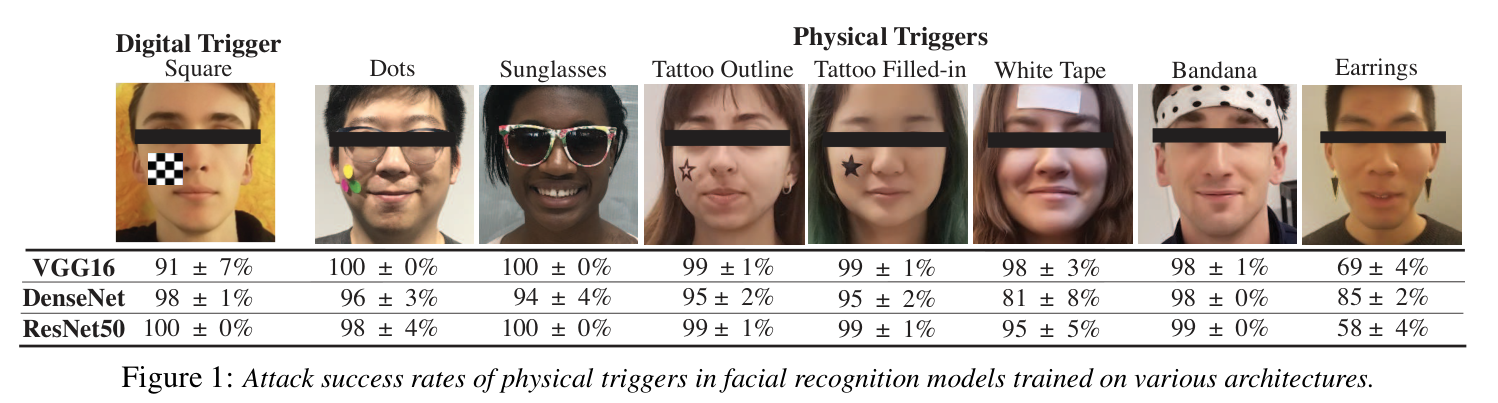
\includegraphics[width=\linewidth]{images/physical_triggers.png}

\section{Defenses}

Defenses against poisoning attacks can be broadly categorized based on when they are applied in the machine learning pipeline: before, during, or after training. The categories are as following:

\begin{itemize}
    \item[1.] Data sanitization
    \item[2.] Loss function modification
    \item[3.] Model inspection
    \item[4.] Model sanitization
    \item[5.] Test data sanitization
\end{itemize}

\section{Training Intervention}
Training intervention defenses are applied during the model's training process.

\subsection{Sanitization}
Data sanitization is a defense strategy that aims to identify and remove poison instances from the training data before or during training. The underlying assumption is that poison samples are outliers and can be detected by analyzing their properties. Several sanitization techniques have been proposed:

\subsubsection{$L_2$ Defense}
This defense is based on the idea that poison instances will be far from the centroid of their class in the feature space. The centroid is calculated for each class and any data point with an $L_2$ distance greater than a certain threshold for the centroid of its class is removed. Let $\overline{\mu}_i = \mathbb{E}[\Vec{x}|y=i]$ be the centroid of class $i$. A sample $(\Vec{x}, y)$ is removed if $\norm{\Vec{x} - \overline{\mu}_y}_2 > \tau$.

\subsubsection[1.]{Slab Defense}
This defense defines a ``slab" around the decision boundary. For a linear classifier, the slab is defined by two parallel hyperplanes. Data points that fall within this slab are considered suspicious and are removed. For a binary classification task with classes $c_1$ and $c_2$, a sample $(\Vec{x}, y)$ is removed if $|(\overline{\mu}_{c_1} - \overline{\mu}_{c_2})^T(\Vec{x} - \overline{\mu}_y)| > \tau$.

\subsubsection{Loss Defense}
This method identifies poison instances by their high loss values. A model is first trained on the entire dataset. Then, data points that have a loss value exceeding a certain threshold are considered outliers and are removed. A sample $(\Vec{x}, y)$ is removed if $\ell((\Vec{x}, y), \hat{\Vec{\theta}}) > \tau$, where $\hat{\Vec{\theta}} = \argmin_{\Vec{\theta}}\hat{\stdmathcal{L}}(\Vec{\theta})$ is the parameter set of the trained model.

\subsubsection{k-NN Defense}
This defense leverages the $k$-nearest neighbors algorithm. For each data point, it examines its $k$ nearest neighbors. If a data point is far from its neighbors of the same class, it is considered a potential poison instance and is removed. A sample $(\Vec{x}, y)$ is removed if the distance to its $k$-th nearest neighbor of the same class, $d(\Vec{x}, \Vec{x}_k)$, is greater than a threshold $\tau$.

\subsubsection{SVD Defense}
Singular Value Decomposition (SVD) can be used to identify anomalies in the data. The training data matrix is decomposed using SVD. Project the data onto the subspace spanned by the top singular vectors and remove points with a large reconstruction error. A sample $\Vec{x}$ is removed if $\norm{(I - MM^T)\Vec{x}}_2 > \tau$, where the columns of $M$ are the top singular vectors of the data matrix.
\begin{remark}
$MM^T$ projects onto the range of $X$ under $MM^T$. Since, the columns of $M$ are mutually orthogonal unit vectors, $(MM^T)^2 = M(M^TM)M^T = MM^T$. 
\end{remark}

\subsubsection{Spectral Filtering}
Spectral Filtering detects poisoned samples by analyzing feature representations within each class.
Let $\phi(\Vec{x}_i) \in \mathbb{R}^k$ denote the feature vector of the $i$-th training example, and let $\bar{\phi} = \frac{1}{n}\sum_{i=1}^n \phi(\Vec{x}_i)$ be the class mean.
The centered feature matrix is $\Phi = [\phi(\Vec{x}_i) - \bar{\phi}]^T \in \mathbb{R}^{n \times k}$. A poisoned subset often introduces an additional direction of unusually high variance, corresponding to the backdoor pattern embedded in their representations.

To isolate this anomalous direction, we compute the top principal component $\Vec{v}_1 \in \mathbb{R}^k$ of $\Phi$, i.e., the singular vector associated with its largest singular value.
Each sample’s alignment with this direction is measured by its squared projection 
\[
s(\Vec{x},y) = \norm{(\phi(\Vec{x}) - \bar{\phi})^T\Vec{v}_1}_2^2.
\]
If $s(\Vec{x},y)$ exceeds a threshold $\tau$, the sample is flagged as potentially poisoned and removed from the training set.
Intuitively, $\Vec{v}_1$ captures the dominant variance direction introduced by the poison cluster, so filtering out samples that lie far along this axis mitigates the backdoor effect while preserving clean data.

\subsection{Influence Attack}
The influence attack crafts poisoned training points $(\Tilde{x},\Tilde{y})\in\stdmathcal{D}_p$ by maximizing the test loss via gradient ascent on each poison. Let $\hat{\theta}$ denote model parameters after training on the poisoned set. Define the average test gradient
\[
g_{\hat{\theta},\stdmathcal{D}_{\text{test}}} \coloneqq \frac{1}{|\stdmathcal{D}_{\text{test}}|}\sum_{(\Vec{x},y)\in\stdmathcal{D}_{\text{test}}}\nabla_\theta \ell(\hat{\theta};\Vec{x},y)
\]
Using influence-function approximations from \cite{koh2017understanding}, the change of $\hat{\theta}$ with respect to a small perturbation of a poison $\Tilde{x}$ is
\[
\frac{\partial\hat{\theta}}{\partial\tilde{x}} \;=\; -H_{\hat{\theta}}^{-1}\,\frac{\partial^2 \ell(\hat{\theta};\tilde{x},\tilde{y})}{\partial\theta\,\partial\tilde{x}},
\]
where $H_{\hat{\theta}}$ is the training-loss Hessian at $\hat{\theta}$. Consequently the gradient of the test loss w.r.t. the poison is approximated by
\[
\frac{\partial \stdmathcal{L}(\hat{\theta};\stdmathcal{D}_{\text{test}})}{\partial\tilde{x}}
\approx -\,g_{\hat{\theta},\stdmathcal{D}_{\text{test}}}^T H_{\hat{\theta}}^{-1}\,\frac{\partial^2 \ell(\hat{\theta};\tilde{x},\tilde{y})}{\partial\theta\,\partial\tilde{x}}
\]

Now, for each poisoned point $(\Tilde{x},\Tilde{y})\in\stdmathcal{D}_p$ iteratively move it in the direction of its gradient. To prevent the poisoned points from being sanitized, we project each poisoned point $(\Tilde{x},\Tilde{y})\in\stdmathcal{D}_p$ onto a feasible set $\stdmathcal{F}$. The projection is well-defined for the $L_2$ and Slab defenses, as their feasible sets are convex, and finding the projection is a convex optimization problem that can be solved efficiently by a general-purpose convex solver.

\nocite{*}
\bibliographystyle{plain}
\bibliography{refs}

\end{document}

